\renewcommand{\lastmod}{December 7, 2023}
\renewcommand{\chapterauthors}{Markus Lippitz}

\chapter{Polarization and anisotropic media}



\goal{By the end of this chapter you should be able to explain and experimentally demonstrate the operation of a wave plate.}


\section{Overview}

Polarization is the most important property of light. It makes the difference to scalar waves. It gives an additional degree of freedom in optical devices. We first introduce the Jones formalism to describe the state of polarization and then discuss the propagation of light in anisotropic media. The most surprising effect is probably birefringence. The technical applications are components of polarization optics such as waveplates and polarizing prisms. Spectroscopic applications include the magneto-optical Kerr effect and circular dichroism.


\section{Introduction}

\begin{marginfigure}
    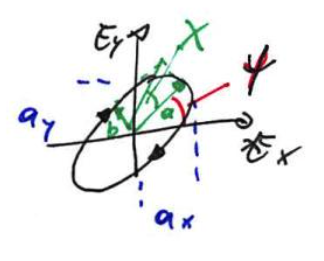
\includegraphics[width=40mm]{\currfiledir sketches/pol_field.png}
    \caption{Electric field in the $xy$-plane.}
\end{marginfigure}

We start by looking at a monochromatic plane wave again. This time, however, we pay more attention to the vectorial amplitude by writing
\begin{equation}
    \bE(z,t) = \Re \left\{ 
    \left( A_x \hat{\bx} + A_y \hat{\by} \right) \, e^{i \omega (t - z/c)}
    \right\}
\end{equation}
where $A_{x,y}$ are complex-valued amplitudes. We separate them intro amplitude $a$ and phase $\phi$ (and write down only the $x$ components for simplicity)
\begin{equation}
    A_x = a_x e^{i \phi_x}
\end{equation}
so that the $x$ components of the field is
\begin{equation}
    E_x = a_x \cos \left( \omega (t - z/c) + \phi_x \right) \quad .
\end{equation}
In the $xy$-plane this describes as function of time $t$ an ellipse with ellipticity $\chi$ and orientation $\psi$:
\begin{align}
    \tan 2 \psi = & \frac{2 R}{1 - R^2} \cos (\phi_y - \phi_x) \\
    \sin 2 \psi = & \frac{2 R}{1 - R^2} \sin (\phi_y - \phi_x) 
\end{align}
with $R = a_y / a_x$.

\begin{questions}
    \item Draw the field $\bE$ for a fixed $t$ in the $xyz$-cube and for a fixed $z$ in the $xyt$-cube.
\end{questions}


\section{Polarization states}

\emph{Linear polarization} is described by
\begin{equation}
    \phi_y - \phi_y = 0 \text{ or } \pi
\end{equation}
In these cases, the ellipticity vanishes $\chi = 0$ and the orientation $\psi$ is 
\begin{equation}
    \tan 2 \psi = \frac{2R}{1 - R^2} \quad \text{or} \quad \tan \psi = \frac{a_y}{a_x} \quad .
\end{equation} 
%
\emph{Circular polarization} is described by
\begin{equation}
    \phi_y - \phi_y = \pm \frac{\pi}{2} \quad \text{and} \quad a_x = a_y
\end{equation}
The electric field vector describes a circle in the $xy$-plane. The plus sign corresponds to right-circularly polarized (RCP), the minus sign to left-circularly polarized (LCP). A snapshot in time gives in the $xyz$ cube a helix of the corresponding\sidenote{This sign differs in some books!} handedness.

All other polarization states can be depicted as point on the \emph{Poincaré sphere}. We need only two parameters to describe the state of polarization, $\chi$ and $\psi$, or $R$ and $\phi_y - \phi_x$. For the Poincaré sphere, we set 
\begin{equation}
    r = 1 \qquad \theta = \frac{\pi}{2} - 2 \chi \qquad \psi = 2 \chi
\end{equation}
North and south pole correspond to RCP and LCP, respectively. The equator describes linearly polarized light ($\chi =  0$) in the different directions.

\begin{marginfigure}
    \includegraphics[width=50mm]{\currfiledir sketches/poincare.png}
    \caption{Polarization states on the Poincaré sphere.}
\end{marginfigure}

A more general method to describe polarized light is the four-component \emph{Stokes vector}. The first component is the intensity of the light field that was not contained in the Poincaré sphere. The other three are the three cartesian components of the point on the Poincaré sphere, i.e.
\begin{align}
    S_0 = & a_x^2 + a_y^2 \\
    S_1 = & a_x^2 - a_y^2 \\
    S_2 = & 2 a_x  a_y \cos (\phi_y - \phi_x )\\
    S_3 = & 2 a_x  a_y \sin (\phi_y - \phi_x )
\end{align}
As we have introduced the $a_{x,y}$ above, we always get $S_1^2 + S_2^2 + S_3^2 = 1$, which would not justify an additional component. However, the scheme can be extended to describe partially polarized or unpolarized light, for which the last component is needed.



\section{Jones formalism}

The simplest way to describe the effect of optical elements such as quarter and half wave plates or polarizers on the polarization state of light is the Jones formalism. We write the complex amplitudes $A_x$ and $A_y$ as the two components of a Jones vector
\begin{equation}
    \bJ = \begin{pmatrix}
        A_x \\ A_y
    \end{pmatrix}
\end{equation}
In most cases we normalize $|\bJ| = 1$. Examples are 
\begin{equation}
    \begin{pmatrix}
       1 \\ 0
    \end{pmatrix} 
    \qquad 
      \begin{pmatrix}
        \cos \theta \\ \sin \theta
     \end{pmatrix}
     \qquad
     \frac{1}{\sqrt{2}}
     \begin{pmatrix}
        1 \\ i
     \end{pmatrix} 
     \qquad 
     \frac{1}{\sqrt{2}}
     \begin{pmatrix}
        1 \\ -i
     \end{pmatrix} 
\end{equation}
for linear polarization in x direction, under an angle $\theta$ to the x-direction, and right and left-handed circular polarization.

A $2 \times 2$ matrix describes the effect of an optical element. A \emph{linear polarizer} is
\begin{equation}
    T = 
    \begin{pmatrix}
   1 & 0 \\ 0 & 0
    \end{pmatrix} 
\end{equation}
A \emph{wave plate} delays the slow y component by a phase $\phi$ compared to the fast x component, i.e.
\begin{equation}
    T = 
    \begin{pmatrix}
   1 & 0 \\ 0 & e^{-i \phi}
    \end{pmatrix} 
\end{equation}
As light travels faster when polarized along the x axis, it is called the 'fast axis' of the wave plate.
Important cases are the quarter-wave plate with $\phi = \pi/2 = 2 \pi / 4$ and the half-wave plate with  $\phi = \pi = 2 \pi / 2$. A \emph{quarter wave plate} converts linear polarized light under $45^\circ $ into LCP, and RCP in linear polarized light under $45^\circ$:
\begin{equation}
    \begin{pmatrix}
        1 \\ -i
     \end{pmatrix}
     = 
    \begin{pmatrix}
        1 & 0 \\ 0 & e^{-i \pi/2}
         \end{pmatrix} \cdot
         \begin{pmatrix}
            1 \\ 1
         \end{pmatrix}
         \quad \text{and} \quad
         \begin{pmatrix}
            1 \\ 1
         \end{pmatrix}
         = 
        \begin{pmatrix}
            1 & 0 \\ 0 & e^{-i \pi/2}
             \end{pmatrix} \cdot
             \begin{pmatrix}
                1 \\ i
             \end{pmatrix}
\end{equation}
A \emph{half wave plate converts} turns the polarization direction of
linear polarized light from $+45^\circ $ to $-45^\circ $, i.e., by $90^\circ$. It also converts RCP into LCP:
\begin{equation}
            \begin{pmatrix}
                1 \\ -1
             \end{pmatrix}
             = 
            \begin{pmatrix}
                1 & 0 \\ 0 & e^{-i \pi}
                 \end{pmatrix} \cdot
                 \begin{pmatrix}
                    1 \\ 1
                 \end{pmatrix}
                 \quad \text{and} \quad
                 \begin{pmatrix}
                    1 \\ -i
                 \end{pmatrix}
                 = 
                \begin{pmatrix}
                    1 & 0 \\ 0 & e^{-i \pi}
                     \end{pmatrix} \cdot
                     \begin{pmatrix}
                        1 \\ i
                     \end{pmatrix}
\end{equation}
It is important to note that these conversions only work for the indicated relative orientation of the waves plates x and y axis and the incoming polarization state. In almost all cases, one needs to rotate the  optical elements relative to the lab-frame $xy$ coordinate system. The effect of a rotated element $T'(\theta)$ is obtained by rotation matrices
\begin{equation}
    T'(\theta) = R(\theta) \cdot T \cdot R(-\theta) \quad \text{with} \quad
    R(\theta) = 
    \begin{pmatrix}
        \cos \theta & \sin \theta \\ 
        - \sin \theta & \cos \theta 
    \end{pmatrix}
\end{equation}

\begin{questions}
    \item Find orientations of quarter- and half-wave plate that do not change a linearly polarized beam!
    \item Plot the total power in a beam as function of angle $\theta$ of a linear polarizer relative to a linear polarized beam and to a left-circular polarized beam.
\end{questions}


\section{Anisotropic media} 

The refractive index of anisotropic media depends on the polarization direction of the light wave. This statement defines anisotropic media. This relationship makes anisotropic media of special interest for polarization optics, and polarization optics of importance for the study of anisotropic media. Before we get to the propagation of light in anisotropic media, let us discuss the microscopic patterns of  anisotropy. On the nanoscale, molecules could be ordered in position and / or orientation.
\begin{description}
    \item[gases, liquids, amorphous solids] Both position and orientation are random. The media are isotropic
    \item[polycrystallline solids] On a short length scale we find order in position and orientation, leading to anisotropy. On a longer length scale, the crystallites are disordered, averaging out the anisotropy. 
    \item[crystalls] Both position and direction are ordered. In general case, crystals are anisotropic. 
    \item[liquid crystals] The position is random, but the orientation is ordered. This is enough to find anisotropy. 
\end{description}

\begin{marginfigure}
    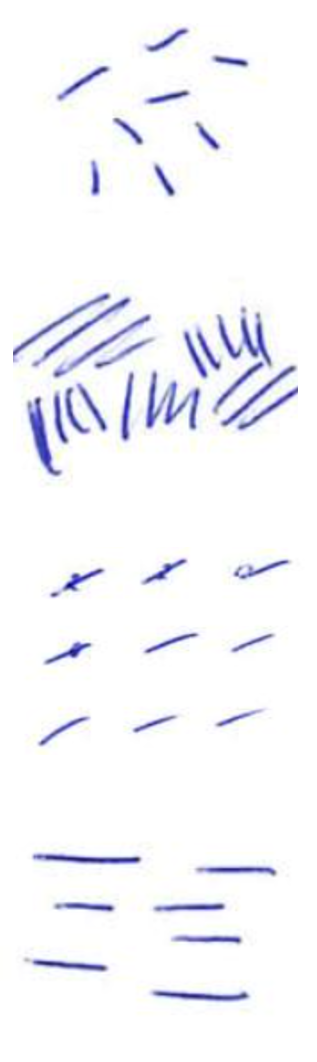
\includegraphics[width=30mm]{\currfiledir sketches/order.png}
    \caption{Order in position and / or orientation.}
\end{marginfigure}



\section{Index ellipsoid }

When we deal with anisotropic media, we have to take the tensorial nature of the electric permittivity $\beps$ into account:
\begin{equation}
   \bD = \epsilon_0 \beps \bE \quad \text{or} \quad  D_i = \epsilon_0 \sum_j \epsilon_{i j} \, E_j \quad \text{with} \quad i,j = x, y, z  \label{eq:5_eps_trensor}
\end{equation}
where $\epsilon_{i j} $ are the components of the $3\times 3$ tensor $\beps$. For most materials, the tensor is symmetric, i.e., $\epsilon_{ij} = \epsilon_{ji}$.  This holds for nonmagnetic dielectrics that do not show optical activity, and in absence of magnetic fields. The symmetry reduces the originally 9 elements to 6 independent ones.\sidenote{see chapter 15.4 of \cite{Brooker_Optics} for an interpretation of the coefficients}

We can depict such a symmetric tensor as ellipsoidal surface defined by 
\begin{equation}
     \sum_{i,j} \epsilon_{i j}  x_i x_j = 1
\end{equation}
When we change the coordinate system, then both the $x_i$ and the $\epsilon_{ij}$ change and the ellipsoid remains unchanged. There is one coordinate system in which the $\epsilon_{ij}$ matrix is diagonal. This are the principal axes.  In these directions, $\bE$ amd $nD$ are parallel. In the following, my spatial coordinate system is always this principal system, labeled as $x_1$, $x_2$, $x_3$ The semi-axes of the ellipsoid, i.e., where the ellipsoid crosses the axes, have the values $1/\sqrt{\epsilon_i} = 1/n_i$. Here $n_i$ is the index of refraction along one of the principal axes.


\begin{marginfigure}
    \inputtikz{\currfiledir ellipsoid}
    \caption{The index ellipsoid for an uniaxial crystal.}
\end{marginfigure}


In the following, it is more useful to have the inverse tensor $\boldsymbol{\eta} = \beps^{-1}$, i.e.
\begin{equation}
    \bE = \frac{1}{\epsilon_0} \beps^{-1} \bD  = \frac{\boldsymbol{\eta}}{\epsilon_0}  \bD
 \end{equation}
When depicted as ellipsoid, called \emph{index ellipsoid}, its principal axes agree with the permittivity tensor. The intersections with the axes are at $n_i$ and we can write
\begin{equation}
    \sum_{i=1,2,3} \frac{x_i^2}{n_i^2} = 1
\end{equation}



We distinguish crystals by their set of $n_i$:
\begin{align}
          &  n_1 = n_2 = n_3             & & \quad \text{isotropic} \\
 n_{o} = &  n_1 = n_2  \neq n_3  =n_{eo} && \quad \text{uniaxial} \\
           &   n_1 \neq n_2  \neq n_3      & & \quad \text{biaxial} 
\end{align}
In this chapter, we will only discuss  uniaxial crystals. Their two index values are called 'ordinary' and 'extraordinary'. The principal axis of the third, extraordinary value is called 'optics axis', not to be confused with the optical\sidenote{In German, both is 'optische Achse'!} axis ($=z$).



\section{Propagation along a principal axis}

Let us start discussing the propagation of light in anisotropic media by assuming that we travel along a principal axis. This means that the wavevector $\bk$ is parallel to one of the $x_i$. When the electric field $\bE$ is parallel to another principal $x_j$, then also $\bD$ remains parallel to $x_j$. The wave travels as in an homogenous medium with index of refraction $n_j$ and the state of polarization remains unchanged.

When the direction of the electric field does not coincide with one of the $x_i$, then we can write it as superposition of fields along several $x_i$. Each of these fields travels as above, but  experiences a different index of refraction. After a distance $d$ they  have acquired a phase difference of 
\begin{equation}
    \Delta \phi = \Delta n \, k_0 \, d
\end{equation}
This is what a wave plate is doing. A uniaxial crystal is cut such that the in-plane directions have a different index of refraction.


\section{Propagation along an arbitrary direction}

Now the plane wave is allowed to travel in any direction $\bk$. It is not constrained to a principal axis as above. We draw\sidenote{see \cite{SalehTeich1991} for a proof that this works} the wave vector $\bk$ in the index ellipsoid and construct a plane perpendicular to it that contains the origin of the coordinate system. The ellipsoid crosses this plane, forming an \emph{index ellipse}. The principal axes of this index ellipse are perpendicular to $\bk$ and describe the two linear polarization directions that propagate unperturbed, i.e. are normal modes. The lengths of the semi-axes of the ellipse give the index of refraction experienced by these two polarization states.


\begin{marginfigure}
    \inputtikz{\currfiledir ellipsoid_cut}
    \caption{When traveling in direction $\boldsymbol{\hat{u}}$, the refractive index of the eigen-modes are found as semi-axes of the ellipse perpendicular to $\boldsymbol{\hat{u}}$ .}
\end{marginfigure}


In the special case of an uniaxial crystal, one wave, the ordinary wave, will always experience the ordinary index of refraction $n_o$. The other, extraordinary  one will experience an index that is a mixture of ordinary and extraordinary. The mixing ratio depends on the angle $\theta$ that the wave vector makes with the optics axis:
\begin{equation}
    \frac{1}{n(\theta)} = \frac{\cos^2 \theta}{n_o^2} + \frac{\sin^2 \theta}{n_{eo}^2}
\end{equation}



\section{Energy flow and wave fronts}

The extraordinary wave is really extraordinary. We will see this when looking at the direction of the Poynting vector. To describe an optical plane wave, we have the wave vector $\bk$, the fields $\bE$, $\bD$, $\bB$, and $\bH$ and the Poynting vector $\bS$. When the spatial variation of all fields is proportional to $\exp(i \bk \cdot \br)$, then Maxwells equations lead to
\begin{align}
    \bk \times \bH = & - \omega \bD  \label{eq:6_kHD}\\
    \bk \times \bE = &  \omega \mu_0 \bH     \label{eq:6_kEH}
\end{align}
This means that $\bk$, $\bH$, and  $\bD$ are perpendicular to each other, and  $\bk$, $\bE$, and $\bH$. The Poynting vector $\bS = \frac{1}{2} \bE \times \bH^\star$ is perpendicular on $\bE$ and $\bH$.

\begin{marginfigure}
    \inputtikz{\currfiledir energy_flow}
    \caption{For an extraordinary wave, Poynting vector $\bS$ and wave vector $\bk$ point in different directions.
    \label{fig:5_energy_flow}}
\end{marginfigure}

For the extraordinary wave, the tensorial nature of $\beps$ does  comes into play: $\bE$ and $\bD$ are not necessarily parallel. Luckily, this is also not  requited by any relation in the last paragraph. Fig.~\ref{fig:5_energy_flow} sketches how the required perpendicularities are resolved with non-parallel  $\bE$ and $\bD$. This means that the wave vector $\bk$ is not parallel anymore to the Poynting vector $\bS$. As the wave fronts are perpendicular to $\bk$, in the case of extraordinary waves, the energy transport ist not perpendicular to the wavefronts anymore! This justifies the label 'extraordinary'. In the following, I will call this object of wavefronts not perpendicular to energy flow a 'beam', in contrast to a plane wave, and similar to a Gaussian beam, in which also the wave fronts are curved and thus not everywhere perpendicular to the energy flow.

Lets look at the direction of energy flow and wave fronts a bit more in detail. We combine the  equations  \ref{eq:6_kHD} and  \ref{eq:6_kEH} with \ref{eq:5_eps_trensor} and get
\begin{equation}
    \bk \times ( \bk \times \bE) + \omega^2 \mu_0 \epsilon_0 \beps \bE = 0
\end{equation}
At a given frequency $\omega$, this is a linear equation system for the thee components of $\bE$. It has a solution if the determinant vanishes. In the case of uniaxial crystals, this reads
\begin{equation}
    (k^2 - n_0^2 k_0^2) \left( \frac{k_1^2 + k_2^2}{n_{eo}^2} + \frac{k_3^2}{n_o^2} - k_0^2  \right) = 0
\end{equation}
This equation describes a surface in the 3d space of $\bk$, the k-surface. In fact, we find two solutions: the first factor becomes zero, leading to a spherical surface related to  the ordinary wave 
\begin{equation}
    | \bk| = k = n_o \, k_0
\end{equation}
The second factor describes an ellipsoid and the extraordinary wave
\begin{equation}
    \frac{k_1^2 + k_2^2}{n_{eo}^2} + \frac{k_3^2}{n_o^2} = k_0^2 
\end{equation}



How does one use these k-surfaces? We start by defining the direction $\boldsymbol{\hat{u}}$ of the wavevector $\bk$. The distance of the surface from the origin in the direction of $\boldsymbol{\hat{u}}$ gives the index of refraction of that wave. This recover its dependence on angle $\theta$ between $\bk$ and the optics axis $x_3$, as discussed in the last section. Additionally, one can show\footcite{SalehTeich1991} that the Poynting vector $\bS$ is perpendicular to the surface at these points. And the wave fronts are perpendicular to $\bk$ and thus $\boldsymbol{\hat{u}}$ as usual.

XXX fig sketches


\section{Birefringence}

The existence of both an ordinary and an extraordinary wave leads to birefringence. A plane wave is diffracted into two different directions when entering an anisotropic material from the air side. Depending on the polarization direction, the wave sees the ordinary index of refraction $n_o$, or the extraordinary $n_{eo}$, where the latter depends on the  angle relative to the optics axis of the crystal. For both polarization directions, Snell's law has to hold, i.e.
\begin{equation}
    \sin \theta_{air} = n_o \sin \theta_o \quad \text{and} \quad   \sin \theta_{air} = n_{eo} \sin \theta_{eo} 
\end{equation}
When $\theta_a$ is the angle of the optics axis with the surface normal, then we can calculate $n_{eo} = n(\theta_a + \theta_{eo})$, using eq. XXX above.

Snell's law describes the direction of the wave vector $\bk$ and the wave fronts, but it does not describe the energy flow or the direction of the Poynting vector $\bS$, at least not in the case of anisotropic media. We see this when letting the plane wave impinge perpendicular on the crystal surface, i.e., set $\theta_{air} = 0$. So also inside the crystal, the wave fronts remain parallel to the crystal surface, all angles remain equal to zero. But the Poynting vector is perpendicular to the k-surface. When the optics axis of the crystal is neither parallel nor perpendicular to the crystal surface, the Poynting vector for the extraordinary beam will deviate. A beam with the extraordinary polarization direction will be displaced in an anisotropic plate. This is used in different types of polarizing beam-splitter prisms.


XXX Fig. 6.32 S/T


XXX discuss pol BS ???

\section{Optical activity and magneto-optics}

I would like to briefly discuss another aspect of anisotropic media. Until now we have assumes that the dielectric tensor $\beps$ is symmetric, i.e. $\epsilon_{ij} = \epsilon_{ji}$. This has led to linear polarization states as eigen-modes, i.e. linearly polarized light travels unperturbed for some polarization directions and directions of travels. Now we do something else. We assume that the dielectric tensor $\beps$ is hermitian, i.e. $\epsilon_{ij} = \epsilon_{ji}^\star$. This leads to circular polarization as eigen-modes. RCP and LCP light travels unperturbed, but with a different index of refraction.

We can write linear polarized light (angie $\theta$) as  superposition of RCP and LCP:
\begin{equation}
    \begin{pmatrix}
        \cos \theta \\ \sin \theta
    \end{pmatrix}
    = 
    \frac{1}{2} e^{-i \theta} 
    \begin{pmatrix}
        1 \\ +i 
    \end{pmatrix}
    +
    \frac{1}{2} e^{+i \theta} 
    \begin{pmatrix}
        1 \\ -i 
    \end{pmatrix}
\end{equation}
After traveling a distance $d$, RCP and LCP waves have accumulated a different phase factor, $\phi_+$ and $\phi_-$
\begin{equation}
    \phi_\pm = 2 \pi n_\pm \frac{d}{\lambda}
\end{equation}
The difference $\phi =\phi_- - \phi_+$ leads to a rotation of the linear polarization state. The resulting Jones vector is
\begin{equation}
    e^{-i (\phi_+ + \phi_-) / 2} 
    \begin{pmatrix}
        \cos \theta  - \phi/2\\ \sin \theta - \phi/2
    \end{pmatrix}
\end{equation}
The 'rotary power' is, for small $\zeta \ll n = \sqrt{\epsilon_{ii}}$
\begin{equation}
    \rho = \frac{\phi/2}{d} \approx - \frac{\pi \zeta}{n \lambda_0}
\end{equation}

Such a tensor is connected with two effects: Optical activity and magneto-optics. Optical active media can be described by 
\begin{equation}
    \bD = \epsilon_0 \epsilon \bE + i \epsilon_0 \boldsymbol{G} \times \bE \quad \text{with} \quad \boldsymbol{G} = \zeta \bk
\end{equation}
with the gyration vector $\boldsymbol{G}$. When the wave travels in z-direction, then only the off-diagonal elements $\epsilon_{12} = i \zeta = \epsilon_{21}^\star$ are different from zero and the diagonal tensor elements are all the same. This can be found in materials with a helical structure, for example quartz, or liquids of chiral molecules, for example amino-acids or sugars.


The Faraday effect is a similar effect in magneto-optics. The dielectric tensor has the same structure, except that the gyration vector is
\begin{equation}
    \boldsymbol{G} = \gamma \bB
\end{equation}
with the gyromagnetic ratio $\gamma$. The fundamental difference is that an optically active medium rotates the direction of polarization as a function of the direction of propagation, while the Faraday effect is a function of the direction of the magnetic field. Consequently, when a wave is reflected and travels back through the same medium, the effect of optical activity is canceled, while the Faraday effect is doubled. Normally, in optics, the direction of travel can be reversed and everything happens in the opposite direction, as we have done when tracing light rays through lenses. When the Faraday effect is involved, this does not work. Running back does not give the starting condition anymore. In this way, one can build an optical diode, the \emph{Faraday isolator}, which allows light to pass only in one direction and prevents, for example, light from being reflected back into a laser cavity.

\section{Hands on: wave plate}

 XXX missing




%--------------------
\printbibliography[segment=\therefsegment,heading=subbibliography]
